\documentclass[12pt,a4paper]{article}
\usepackage[utf8]{vietnam}
\usepackage{amsmath,amssymb,amsfonts}
\usepackage[left=1.5cm,right=1.5cm,top=2cm,bottom=2cm,headheight=17pt]{geometry}
\usepackage{enumitem,array,graphicx,tikz,fancyhdr,needspace}
\usetikzlibrary{arrows.meta,calc,patterns}
\pagestyle{fancy}\fancyhf{}
\lhead{\small\textbf{HƯỚNG TỚI THPTQG 2027}}
\rhead{\small\textit{Người biên soạn: Dương Gia Bảo}}
\rfoot{\small Trang \thepage}
\renewcommand{\headrulewidth}{0.4pt}
\setlength{\parindent}{0pt}\setlength{\parskip}{3pt}
\setlist[enumerate,1]{label=\textbf{Câu \arabic*:},leftmargin=*,itemsep=9pt,topsep=6pt}
\setlist[enumerate,2]{label=\alph*),leftmargin=*,itemsep=3pt,topsep=4pt}
\newcommand{\bonpa}[4]{\par\smallskip\noindent
\begin{tabular}{@{}p{0.47\linewidth}p{0.47\linewidth}@{}}
\textbf{A.} #1 & \textbf{B.} #2\\[3pt]
\textbf{C.} #3 & \textbf{D.} #4\end{tabular}}
\newcommand{\loigiai}[1]{\par\medskip\Needspace{4\baselineskip}\noindent\textbf{#1}\par\nobreak}

\begin{document}
\begin{minipage}[t]{0.40\textwidth}\centering
\textbf{HƯỚNG TỚI THPTQG 2027}\\[-2pt]
\rule{3.2cm}{0.6pt}\\[4pt]\textbf{ĐỀ CHÍNH THỨC}
\end{minipage}\hfill
\begin{minipage}[t]{0.58\textwidth}\centering
\textbf{ĐỀ THI KHẢO SÁT CHẤT LƯỢNG LỚP 12}\\
\textbf{CHUYÊN ĐỀ: KHẢO SÁT HÀM SỐ}\\\textbf{Môn thi: TOÁN}\\
\textit{\small Thời gian làm bài: 90 phút, không kể thời gian phát đề}
\end{minipage}
\vspace{0.2cm}

\noindent
\begin{minipage}[b]{0.78\textwidth}
\textbf{Họ và tên:}\dotfill\textbf{SBD:}\makebox[3.5cm]{\dotfill}
\end{minipage}\hfill
\begin{minipage}[b]{0.20\textwidth}\hfill
\setlength{\fboxrule}{0.8pt}%
\fbox{\begin{minipage}{2.3cm}\centering\textbf{\small Mã đề thi}\\\textbf{0101}\end{minipage}}
\end{minipage}
\vspace{0.2cm}

\section*{\large PHẦN I. CÂU TRẮC NGHIỆM NHIỀU PHƯƠNG ÁN LỰA CHỌN}
\textit{Thí sinh trả lời từ câu 1 đến câu 12. Mỗi câu thí sinh chỉ chọn một phương án. Mỗi câu trả lời đúng được 0,25 điểm.}
\begin{enumerate}
\item Cho hàm số $y = -x^3 + 3x^2 - 4$. Hàm số đã cho đồng biến trên khoảng nào sau đây?
\bonpa{$(-\infty; 0)$.}{$(0; 2)$.}{$(2; +\infty)$.}{$(-1; 3)$.}

\item Cho hàm số $y = x^3 - 3x + 2$. Điểm cực đại của đồ thị hàm số là
\bonpa{$(1; 0)$.}{$(0; 2)$.}{$(-1; 4)$.}{$(-1; 2)$.}

\item Đường tiệm cận đứng của đồ thị hàm số $y = \dfrac{2x - 3}{x + 1}$ là đường thẳng
\bonpa{$x = -1$.}{$y = 2$.}{$x = 1$.}{$y = -3$.}

\item Cho hàm số $y = \dfrac{x^2 - 3x + 5}{x - 2}$. Phương trình đường tiệm cận xiên của đồ thị hàm số là
\bonpa{$y = x + 1$.}{$y = x - 2$.}{$y = x - 1$.}{$y = 2x - 1$.}

\item Giá trị nhỏ nhất của hàm số $f(x) = x^3 - 3x^2 - 9x + 5$ trên đoạn $[0; 4]$ bằng
\bonpa{$-15$.}{$-27$.}{$5$.}{$-22$.}

\item \begin{minipage}[t]{0.56\linewidth}
Đường cong trong hình vẽ bên là đồ thị của hàm số nào dưới đây?
\bonpa{$y = \dfrac{2x+1}{x-1}$.}{$y = \dfrac{2x-1}{x-1}$.}{$y = \dfrac{x+2}{x-1}$.}{$y = \dfrac{2x+1}{x+1}$.}
\end{minipage}\hfill
\begin{minipage}[t]{0.41\linewidth}\vspace{-0.4\baselineskip}\centering
\resizebox{\linewidth}{!}{\begin{tikzpicture}[>=Stealth,scale=0.8,line cap=round,line join=round]
\draw[->] (-3.2,0)--(4.2,0) node[right] {$x$};
\draw[->] (0,-3.2)--(0,4.8) node[above] {$y$};
\node[below left] at (0,0) {$O$};
\draw[dashed,thick,red!70!black] (1,-3.2)--(1,4.5);
\draw[dashed,thick,red!70!black] (-3.2,2)--(4,2);
\node[above left] at (1,0) {$1$};
\node[above left] at (0,2) {$2$};
\draw[blue!65!black,very thick,smooth,samples=100,domain=-3:0.72] plot (\x,{(2*\x+1)/(\x-1)});
\draw[blue!65!black,very thick,smooth,samples=100,domain=1.32:4] plot (\x,{(2*\x+1)/(\x-1)});
\fill (0,-1) circle (2pt) node[left] {$-1$};
\fill (-0.5,0) circle (2pt) node[below left] {$-\frac{1}{2}$};
\end{tikzpicture}}
\end{minipage}

\item Tọa độ tâm đối xứng của đồ thị hàm số $y = \dfrac{2x^2 + 3x - 1}{x + 1}$ là
\bonpa{$I(1; 3)$.}{$I(-1; 1)$.}{$I(-1; -1)$.}{$I(1; -1)$.}

\item Cho hàm số $y = x^3 - 3x^2 + 2$. Số tiếp tuyến của đồ thị hàm số song song với đường thẳng $d: y = 9x - 14$ là
\bonpa{$0$.}{$1$.}{$3$.}{$2$.}

\item Tìm tất cả các giá trị của tham số thực $m$ để hàm số $y = \dfrac{1}{3}x^3 - mx^2 + (m+2)x - 5$ đồng biến trên $\mathbb{R}$.
\bonpa{$-1 \le m \le 2$.}{$m \le -1\text{ hoặc }m \ge 2$.}{$-2 \le m \le 1$.}{$-1 < m < 2$.}

\item Cho hàm số $y = f(x) = x^3 - 3x^2 + 1$. Số nghiệm thực phân biệt của phương trình $2f(x) - 1 = 0$ là
\bonpa{$1$.}{$3$.}{$2$.}{$0$.}

\item Cho hàm số $y = \dfrac{x^2 - x + 1}{x - 1}$. Khoảng cách giữa hai điểm cực trị của đồ thị hàm số bằng
\bonpa{$4$.}{$2\sqrt{5}$.}{$\sqrt{5}$.}{$2\sqrt{2}$.}

\item Một người thợ muốn làm một bể cá bằng kính dạng hình hộp chữ nhật không nắp có thể tích $V = 16\text{ m}^3$. Đáy bể là hình chữ nhật có chiều dài gấp đôi chiều rộng. Giá kính làm đáy bể là $150.000$ đồng/$\text{m}^2$, giá kính làm các mặt xung quanh là $100.000$ đồng/$\text{m}^2$. Chi phí mua kính thấp nhất để hoàn thành bể cá bằng bao nhiêu?
\bonpa{$4{,}2\text{ triệu đồng}$.}{$4{,}8\text{ triệu đồng}$.}{$3{,}2\text{ triệu đồng}$.}{$3{,}6\text{ triệu đồng}$.}
\end{enumerate}

\newpage
\section*{\large PHẦN II. CÂU TRẮC NGHIỆM ĐÚNG SAI}
\textit{Thí sinh trả lời từ câu 1 đến câu 4. Trong mỗi ý a), b), c), d) ở mỗi câu, thí sinh chọn đúng hoặc sai. Thí sinh chọn đúng 1 ý được 0,1 điểm; 2 ý được 0,25 điểm; 3 ý được 0,5 điểm; 4 ý được 1,0 điểm.}
\begin{enumerate}
\item Cho hàm số $y = f(x) = x^3 - 3x^2 - 9x + 2$.
\begin{enumerate}[label=\alph*)]
\item Hàm số đã cho nghịch biến trên khoảng $(-1; 3)$.
\item Hàm số đạt cực tiểu tại điểm $x = -1$.
\item Đồ thị hàm số nhận điểm $I(1; -9)$ làm tâm đối xứng.
\item Trong tất cả các tiếp tuyến của đồ thị hàm số, tiếp tuyến tại tâm đối xứng $I$ có hệ số góc nhỏ nhất bằng $-12$.
\end{enumerate}

\item \begin{minipage}[t]{0.56\linewidth}
Cho hàm số $y = f(x) = \dfrac{x^2 - 2x + 2}{x - 1}$. Đồ thị $(C)$ của hàm số được cho như hình vẽ bên.
\begin{enumerate}[label=\alph*)]
\item Đồ thị hàm số có hai đường tiệm cận là tiệm cận đứng $x = 1$ và tiệm cận xiên $y = x - 1$.
\item Giao điểm của hai đường tiệm cận là điểm $I(1; 0)$.
\item Giá trị cực tiểu của hàm số lớn hơn giá trị cực đại của hàm số.
\item Khoảng cách từ gốc tọa độ $O$ đến đường tiệm cận xiên của đồ thị bằng $1$.
\end{enumerate}
\end{minipage}\hfill
\begin{minipage}[t]{0.41\linewidth}\vspace{-0.4\baselineskip}\centering
\resizebox{\linewidth}{!}{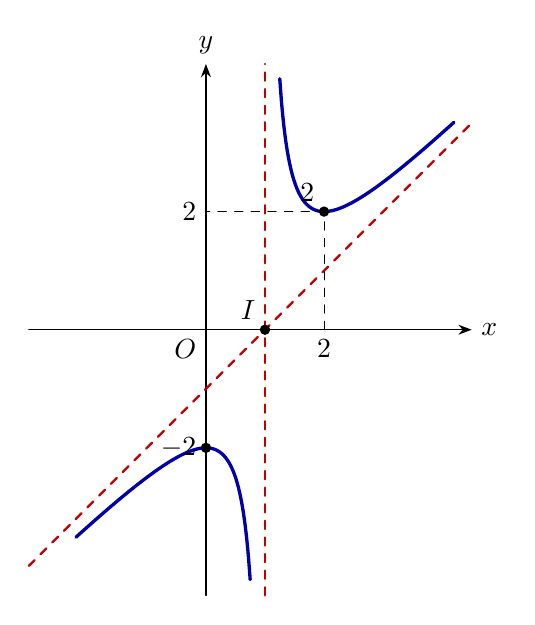
\begin{tikzpicture}[>=Stealth,scale=0.75,line cap=round,line join=round]
\draw[->] (-3,0)--(4.5,0) node[right] {$x$};
\draw[->] (0,-4.5)--(0,4.5) node[above] {$y$};
\node[below left] at (0,0) {$O$};
\draw[dashed,thick,red!75!black] (1,-4.5)--(1,4.5);
\draw[dashed,thick,red!75!black] (-3,-4)--(4.5,3.5);
\draw[blue!65!black,very thick,smooth,samples=100,domain=-2.2:0.75] plot (\x,{(\x*\x - 2*\x + 2)/(\x - 1)});
\draw[blue!65!black,very thick,smooth,samples=100,domain=1.25:4.2] plot (\x,{(\x*\x - 2*\x + 2)/(\x - 1)});
\fill (0,-2) circle (2.5pt) node[left] {$-2$};
\fill (2,2) circle (2.5pt) node[above left] {$2$};
\fill (1,0) circle (2.5pt) node[above left] {$I$};
\draw[dashed] (2,0)--(2,2)--(0,2);
\node[below] at (2,0) {$2$};
\node[left] at (0,2) {$2$};
\end{tikzpicture}}
\end{minipage}

\item Một doanh nghiệp sản xuất độc quyền một loại sản phẩm với sản lượng $x$ sản phẩm mỗi ngày ($x \in \mathbb{N}^*, 1 \le x \le 120$). Giá bán mỗi sản phẩm phụ thuộc vào sản lượng theo hàm số $p(x) = 150 - 0{,}5x$ (nghìn đồng). Tổng chi phí để sản xuất $x$ sản phẩm mỗi ngày được cho bởi hàm số $C(x) = 0{,}25x^2 + 30x + 1200$ (nghìn đồng). Giả sử toàn bộ sản phẩm sản xuất ra đều được tiêu thụ hết.
\begin{enumerate}[label=\alph*)]
\item Hàm doanh thu mỗi ngày của doanh nghiệp là $R(x) = 150x - 0{,}5x^2$ (nghìn đồng).
\item Khi sản xuất và bán $40$ sản phẩm mỗi ngày, doanh nghiệp bị lỗ.
\item Doanh nghiệp đạt lợi nhuận lớn nhất khi sản xuất $80$ sản phẩm mỗi ngày.
\item Lợi nhuận lớn nhất của doanh nghiệp bằng $3{,}6$ triệu đồng mỗi ngày.
\end{enumerate}

\item Một vật chuyển động thẳng với phương trình quãng đường $s(t) = -t^3 + 9t^2 + 21t$ (trong đó $t$ tính bằng giây, $s$ tính bằng mét, với $0 \le t \le 10$).
\begin{enumerate}[label=\alph*)]
\item Vận tốc ban đầu của vật (tại thời điểm $t = 0$) bằng $21\text{ m/s}$.
\item Tại thời điểm gia tốc của vật bằng $0$, vận tốc của vật đạt giá trị lớn nhất.
\item Trong khoảng thời gian từ $t = 0$ đến $t = 7$, vận tốc của vật luôn tăng.
\item Kể từ thời điểm ban đầu, vật dừng lại tại thời điểm $t = 7$ giây.
\end{enumerate}
\end{enumerate}

\newpage
\section*{\large PHẦN III. CÂU TRẮC NGHIỆM TRẢ LỜI NGẮN}
\textit{Thí sinh trả lời từ câu 1 đến câu 6. Mỗi câu trả lời đúng được 0,5 điểm. Chỉ làm tròn ở kết quả cuối cùng.}
\begin{enumerate}
\item Cho hàm số $y = \dfrac{x^2 + 2x - 2}{x - 1}$. Gọi $d_1$ là tiệm cận đứng, $d_2$ là tiệm cận xiên của đồ thị hàm số và $I$ là giao điểm của $d_1, d_2$. Tiếp tuyến bất kỳ của đồ thị hàm số cắt $d_1, d_2$ lần lượt tại $A$ và $B$. Diện tích tam giác $IAB$ bằng bao nhiêu?

\item Tìm tất cả các giá trị nguyên của tham số $m \in [-20; 20]$ để hàm số $y = \dfrac{x^2 - 2mx + 3m - 2}{x - 1}$ đồng biến trên từng khoảng xác định của nó.

\item \begin{minipage}[t]{0.56\linewidth}
Người ta gò một chiếc máng dẫn nước có mặt cắt ngang là hình thang cân $ABCD$ như hình vẽ bên, với đáy nhỏ $BC = 20\text{ cm}$, hai thành bên $AB = CD = 20\text{ cm}$. Góc nghiêng $\alpha$ (tính bằng độ, $0^\circ < \alpha < 90^\circ$) giữa thành bên và phương nằm ngang của đáy để diện tích mặt cắt ngang của máng nước là lớn nhất bằng bao nhiêu độ?
\end{minipage}\hfill
\begin{minipage}[t]{0.41\linewidth}\vspace{-0.4\baselineskip}\centering
\resizebox{\linewidth}{!}{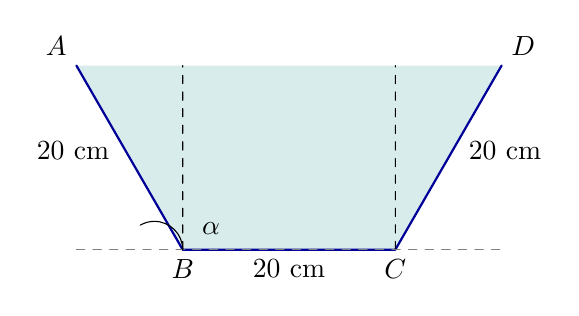
\begin{tikzpicture}[>=Stealth,scale=0.9,line cap=round,line join=round]
\coordinate (B) at (1.5,0);
\coordinate (C) at (4.5,0);
\coordinate (A) at (0,2.598);
\coordinate (D) at (6,2.598);
\fill[teal!15] (A)--(B)--(C)--(D)--cycle;
\draw[thick,blue!60!black] (A)--(B)--(C)--(D);
\draw[dashed] (B)--(1.5,2.598) (C)--(4.5,2.598);
\draw[dashed,gray] (0,0)--(6,0);
\draw (B) arc[start angle=0,end angle=120,radius=0.4];
\node at (1.9,0.3) {$\alpha$};
\node[below] at (3,0) {$20\text{ cm}$};
\node[left] at (0.6,1.4) {$20\text{ cm}$};
\node[right] at (5.4,1.4) {$20\text{ cm}$};
\node[above left] at (A) {$A$};
\node[below] at (B) {$B$};
\node[below] at (C) {$C$};
\node[above right] at (D) {$D$};
\end{tikzpicture}}
\end{minipage}

\item \begin{minipage}[t]{0.56\linewidth}
Một hòn đảo ở vị trí $C$ cách bờ biển thẳng một khoảng $CD = 6\text{ km}$ ($D$ là hình chiếu vuông góc của $C$ lên đường bờ biển). Một trạm phát điện đặt tại điểm $A$ trên bờ biển cách $D$ một khoảng $AD = 9\text{ km}$. Người ta kéo đường dây điện từ $A$ đến một điểm $S$ trên bờ biển (nằm giữa $A$ và $D$) rồi từ $S$ đặt cáp ngầm dưới biển đến đảo $C$. Chi phí kéo $1\text{ km}$ đường dây điện trên đất liền là $30$ triệu đồng, chi phí đặt $1\text{ km}$ cáp ngầm dưới biển là $50$ triệu đồng. Để tổng chi phí kéo dây là nhỏ nhất thì điểm $S$ phải cách trạm $A$ bao nhiêu km?
\end{minipage}\hfill
\begin{minipage}[t]{0.41\linewidth}\vspace{-0.4\baselineskip}\centering
\resizebox{\linewidth}{!}{\begin{tikzpicture}[>=Stealth,scale=0.8,line cap=round,line join=round]
\coordinate (A) at (0,0);
\coordinate (D) at (6,0);
\coordinate (C) at (6,4);
\coordinate (S) at (3,0);
\fill[cyan!12] (-0.5,0) rectangle (7.2,4.5);
\fill[orange!15] (-0.5,-1) rectangle (7.2,0);
\node at (1,3.5) {\textit{Biển}};
\node at (1,-0.5) {\textit{Đất liền}};
\draw[thick] (-0.5,0)--(7.2,0) node[above left] {bờ biển};
\draw[dashed] (C)--(D);
\draw[red!80!black,line width=1.5pt] (A)--(S);
\draw[blue!70!black,line width=1.5pt] (S)--(C);
\fill (A) circle (2.5pt) node[below] {$A$};
\fill (D) circle (2.5pt) node[below] {$D$};
\fill (S) circle (2.5pt) node[below] {$S$};
\fill (C) circle (2.5pt) node[above] {$C$};
\draw[<->] (0,-0.7)--(6,-0.7) node[midway,fill=orange!15] {$9\text{ km}$};
\draw[<->] (6.5,0)--(6.5,4) node[midway,right,fill=cyan!12] {$6\text{ km}$};
\end{tikzpicture}}
\end{minipage}

\item Cho hàm số $y = \dfrac{x^2 + x + 1}{x + 1}$. Xét hai điểm $M, N$ thay đổi trên đồ thị hàm số sao cho $x_M < -1 < x_N$ (nghĩa là $M, N$ thuộc hai nhánh khác nhau của đồ thị). Khoảng cách nhỏ nhất giữa hai điểm $M$ và $N$ bằng bao nhiêu? \textit{(Làm tròn kết quả đến hàng phần trăm.)}

\item \begin{minipage}[t]{0.56\linewidth}
Một tấm biển quảng cáo có chiều cao $AB = 3\text{ m}$ được gắn thẳng đứng trên một bức tường phẳng, sao cho mép dưới $B$ của biển cách mặt đất $2{,}6\text{ m}$. Một người quan sát có tầm mắt $E$ cao $1{,}6\text{ m}$ so với mặt đất, đứng cách tường một khoảng $x$ (mét) để ngắm nhìn tấm biển quảng cáo như hình vẽ bên. Người đó cần đứng cách tường một khoảng bằng bao nhiêu mét để góc quan sát $\theta = \widehat{AEB}$ là lớn nhất?
\end{minipage}\hfill
\begin{minipage}[t]{0.41\linewidth}\vspace{-0.4\baselineskip}\centering
\resizebox{\linewidth}{!}{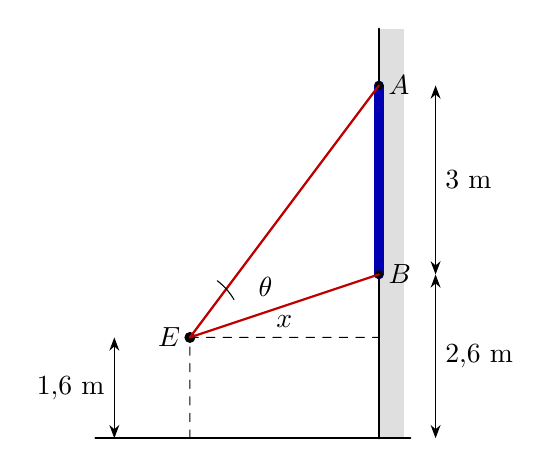
\begin{tikzpicture}[>=Stealth,scale=0.8,line cap=round,line join=round]
\fill[gray!25] (4,0) rectangle (4.4,6.5);
\draw[thick] (4,0)--(4,6.5);
\draw[thick] (-0.5,0)--(4.5,0);
\draw[line width=3.5pt,blue!70!black] (4,2.6)--(4,5.6);
\fill (4,5.6) circle (2pt) node[right] {$A$};
\fill (4,2.6) circle (2pt) node[right] {$B$};
\coordinate (E) at (1,1.6);
\fill (E) circle (2.5pt) node[left] {$E$};
\draw[dashed] (1,0)--(E);
\draw[dashed] (E)--(4,1.6) node[midway,above] {$x$};
\draw[thick,red!75!black] (E)--(4,5.6);
\draw[thick,red!75!black] (E)--(4,2.6);
\draw (1.7,2.2) arc[start angle=30,end angle=53,radius=1];
\node at (2.2,2.4) {$\theta$};
\draw[<->] (4.9,2.6)--(4.9,5.6) node[midway,right] {$3\text{ m}$};
\draw[<->] (-0.2,0)--(-0.2,1.6) node[midway,left] {$1{,}6\text{ m}$};
\draw[<->] (4.9,0)--(4.9,2.6) node[midway,right] {$2{,}6\text{ m}$};
\end{tikzpicture}}
\end{minipage}
\end{enumerate}

\begin{center}\textbf{--- HẾT ---}\end{center}

\newpage
\begin{center}{\Large\textbf{BẢNG ĐÁP ÁN TỔNG HỢP}}\\[4pt]
\textbf{CHUYÊN ĐỀ: KHẢO SÁT HÀM SỐ - MÃ ĐỀ 0101}\end{center}

\textbf{PHẦN I. TRẮC NGHIỆM NHIỀU PHƯƠNG ÁN}
\begin{center}\renewcommand{\arraystretch}{1.5}\begin{tabular}{|*{12}{c|}}\hline
1 & 2 & 3 & 4 & 5 & 6 & 7 & 8 & 9 & 10 & 11 & 12\\\hline
B & C & A & C & D & A & C & D & A & B & B & D\\\hline
\end{tabular}\end{center}

\textbf{PHẦN II. TRẮC NGHIỆM ĐÚNG SAI}
\begin{center}\renewcommand{\arraystretch}{1.5}\begin{tabular}{|c|c|c|c|c|}\hline
Câu & a) & b) & c) & d)\\\hline
1 & Đ & S & Đ & Đ\\\hline
2 & Đ & Đ & Đ & S\\\hline
3 & Đ & S & Đ & Đ\\\hline
4 & Đ & Đ & S & Đ\\\hline
\end{tabular}\end{center}

\textbf{PHẦN III. TRẮC NGHIỆM TRẢ LỜI NGẮN}
\begin{center}\renewcommand{\arraystretch}{1.5}\begin{tabular}{|c|c|c|c|c|c|}\hline
1 & 2 & 3 & 4 & 5 & 6\\\hline
2 & 22 & 60 & 4,5 & 4,39 & 2\\\hline
\end{tabular}\end{center}

\newpage
\begin{center}{\Large\textbf{HƯỚNG DẪN GIẢI CHI TIẾT}}\\[4pt]
\textbf{CHUYÊN ĐỀ: KHẢO SÁT HÀM SỐ - MÃ ĐỀ 0101}\end{center}

\section*{\large PHẦN I. TRẮC NGHIỆM NHIỀU PHƯƠNG ÁN}
\loigiai{Câu 1. Chọn B.}
Ta có đạo hàm $y' = -3x^2 + 6x = -3x(x - 2)$.\\
Cho $y' > 0 \iff -3x(x - 2) > 0 \iff 0 < x < 2$.\\
Vậy hàm số đồng biến trên khoảng $(0; 2)$.

\loigiai{Câu 2. Chọn C.}
Tập xác định $D = \mathbb{R}$. Đạo hàm $y' = 3x^2 - 3$.\\
Cho $y' = 0 \iff x = \pm 1$. Ta có $y'' = 6x \implies y''(-1) = -6 < 0$ nên $x = -1$ là điểm cực đại của hàm số.\\
Tại $x = -1 \implies y = (-1)^3 - 3(-1) + 2 = 4$. Điểm cực đại của đồ thị hàm số là $(-1; 4)$.

\loigiai{Câu 3. Chọn A.}
Vì $\displaystyle\lim_{x \to -1^+} \dfrac{2x - 3}{x + 1} = -\infty$ và $\displaystyle\lim_{x \to -1^-} \dfrac{2x - 3}{x + 1} = +\infty$ nên đường thẳng $x = -1$ là tiệm cận đứng của đồ thị hàm số.

\loigiai{Câu 4. Chọn C.}
Chia đa thức tử cho mẫu ta được:
\[y = \dfrac{x^2 - 3x + 5}{x - 2} = x - 1 + \dfrac{3}{x - 2}.\]
Vì $\displaystyle\lim_{x \to \pm\infty} [y - (x - 1)] = \lim_{x \to \pm\infty} \dfrac{3}{x - 2} = 0$ nên đường tiệm cận xiên của đồ thị là $y = x - 1$.

\loigiai{Câu 5. Chọn D.}
Đạo hàm $f'(x) = 3x^2 - 6x - 9 = 3(x + 1)(x - 3)$.\\
Trên đoạn $[0; 4]$, $f'(x) = 0 \iff x = 3$ (loại điểm $x = -1$).\\
Tính các giá trị tại đầu mút và điểm dừng:
\[f(0) = 5,\quad f(3) = 3^3 - 3(3^2) - 9(3) + 5 = -22,\quad f(4) = 4^3 - 3(4^2) - 9(4) + 5 = -15.\]
Vậy $\displaystyle\min_{[0; 4]} f(x) = -22$.

\loigiai{Câu 6. Chọn A.}
Từ đồ thị hàm số ta nhận thấy:
\begin{itemize}
\item Đường tiệm cận đứng là $x = 1$, đường tiệm cận ngang là $y = 2$.
\item Đồ thị cắt trục tung tại điểm $(0; -1)$ và cắt trục hoành tại điểm $\left(-\dfrac{1}{2}; 0\right)$.
\end{itemize}
Xét hàm số $y = \dfrac{2x+1}{x-1}$: có TCĐ $x = 1$, TCN $y = 2$, cho $x = 0 \implies y = -1$ thỏa mãn toàn bộ các đặc trưng của đồ thị.

\loigiai{Câu 7. Chọn C.}
Thực hiện phép chia: $y = \dfrac{2x^2 + 3x - 1}{x + 1} = 2x + 1 - \dfrac{2}{x + 1}$.\\
Đồ thị hàm số có tiệm cận đứng là $d_1: x = -1$ và tiệm cận xiên là $d_2: y = 2x + 1$.\\
Tâm đối xứng của đồ thị là giao điểm $I$ của hai đường tiệm cận:
\[x_I = -1 \implies y_I = 2(-1) + 1 = -1 \implies I(-1; -1).\]

\loigiai{Câu 8. Chọn D.}
Đạo hàm $y' = 3x^2 - 6x$.\\
Đường thẳng $d: y = 9x - 14$ có hệ số góc bằng $9$. Tiếp tuyến song song với $d$ thỏa mãn:
\[y'(x_0) = 9 \iff 3x_0^2 - 6x_0 - 9 = 0 \iff x_0^2 - 2x_0 - 3 = 0 \iff \left[\begin{aligned}&x_0 = -1\\&x_0 = 3\end{aligned}\right.\]
\begin{itemize}
\item Với $x_0 = -1 \implies y_0 = -2$. Phương trình tiếp tuyến là: $y = 9(x + 1) - 2 = 9x + 7$ (thỏa mãn song song với $d$).
\item Với $x_0 = 3 \implies y_0 = 2$. Phương trình tiếp tuyến là: $y = 9(x - 3) + 2 = 9x - 25$ (thỏa mãn song song với $d$).
\end{itemize}
Vậy có đúng $2$ tiếp tuyến thỏa mãn yêu cầu đề bài.

\loigiai{Câu 9. Chọn A.}
Tập xác định $D = \mathbb{R}$. Ta có $y' = x^2 - 2mx + m + 2$.\\
Hàm số đồng biến trên $\mathbb{R}$ khi và chỉ khi $y' \ge 0$ với mọi $x \in \mathbb{R}$.\\
Vì hệ số của $x^2$ là $1 > 0$, điều này tương đương:
\[\Delta' \le 0 \iff (-m)^2 - (m + 2) \le 0 \iff m^2 - m - 2 \le 0 \iff -1 \le m \le 2.\]

\loigiai{Câu 10. Chọn B.}
Phương trình $2f(x) - 1 = 0 \iff f(x) = \dfrac{1}{2}$.\\
Xét hàm số $f(x) = x^3 - 3x^2 + 1$: $f'(x) = 3x^2 - 6x = 0 \iff x = 0$ hoặc $x = 2$.\\
Bảng biến thiên cho thấy điểm cực đại là $(0; 1)$ và điểm cực tiểu là $(2; -3)$.\\
Vì $-3 < \dfrac{1}{2} < 1$ nên đường thẳng $y = \dfrac{1}{2}$ cắt đồ thị tại đúng $3$ điểm phân biệt. Vậy phương trình có $3$ nghiệm thực phân biệt.

\loigiai{Câu 11. Chọn B.}
Ta có $y = x + \dfrac{1}{x - 1} \implies y' = 1 - \dfrac{1}{(x-1)^2} = \dfrac{x(x-2)}{(x-1)^2}$.\\
Cho $y' = 0 \iff x = 0$ hoặc $x = 2$.\\
Với $x = 0 \implies y = -1$, ta được điểm cực đại $A(0; -1)$.\\
Với $x = 2 \implies y = 3$, ta được điểm cực tiểu $B(2; 3)$.\\
Khoảng cách giữa hai điểm cực trị:
\[AB = \sqrt{(2 - 0)^2 + (3 - (-1))^2} = \sqrt{4 + 16} = \sqrt{20} = 2\sqrt{5}.\]

\loigiai{Câu 12. Chọn D.}
Gọi chiều rộng đáy bể là $x$ (m, $x > 0$). Chiều dài đáy bể là $2x$ (m).\\
Gọi chiều cao của bể cá là $h$ (m, $h > 0$). Thể tích bể là:
\[V = 2x \cdot x \cdot h = 2x^2 h = 16 \implies h = \dfrac{8}{x^2}.\]
Diện tích đáy bể là $S_{\text{đáy}} = 2x^2$ ($\text{m}^2$).\\
Diện tích xung quanh là $S_{\text{xq}} = 2(x + 2x)h = 6xh = 6x \cdot \dfrac{8}{x^2} = \dfrac{48}{x}$ ($\text{m}^2$).\\
Tổng chi phí làm bể kính (đơn vị: nghìn đồng) là:
\[C(x) = 150 \cdot 2x^2 + 100 \cdot \dfrac{48}{x} = 300x^2 + \dfrac{4800}{x}.\]
Đạo hàm: $C'(x) = 600x - \dfrac{4800}{x^2} = \dfrac{600(x^3 - 8)}{x^2}$.\\
Cho $C'(x) = 0 \iff x = 2$ (m).\\
Bảng biến thiên cho thấy $C(x)$ đạt giá trị nhỏ nhất tại $x = 2$:
\[C(2) = 300(2^2) + \dfrac{4800}{2} = 1200 + 2400 = 3600\text{ (nghìn đồng)} = 3{,}6\text{ triệu đồng}.\]

\Needspace{10\baselineskip}
\section*{\large PHẦN II. TRẮC NGHIỆM ĐÚNG SAI}
\loigiai{Câu 1. a) Đúng; b) Sai; c) Đúng; d) Đúng.}
Ta có $f'(x) = 3x^2 - 6x - 9 = 3(x + 1)(x - 3)$ và $f''(x) = 6x - 6$.
\begin{itemize}
\item[a)] $f'(x) < 0 \iff -1 < x < 3$, do đó hàm số nghịch biến trên khoảng $(-1; 3)$. Ý a) Đúng.
\item[b)] Qua điểm $x = -1$, đạo hàm $f'(x)$ đổi dấu từ dương sang âm nên $x = -1$ là điểm cực đại (còn $x = 3$ mới là điểm cực tiểu). Ý b) Sai.
\item[c)] Cho $f''(x) = 0 \iff 6x - 6 = 0 \iff x = 1 \implies y(1) = 1 - 3 - 9 + 2 = -9$. Đồ thị hàm số bậc ba luôn nhận điểm uốn $I(1; -9)$ làm tâm đối xứng. Ý c) Đúng.
\item[d)] Hệ số góc của tiếp tuyến tại điểm có hoành độ $x$ là $k(x) = f'(x) = 3x^2 - 6x - 9 = 3(x - 1)^2 - 12 \ge -12$. Dấu bằng xảy ra khi $x = 1$, chính là hoành độ của tâm đối xứng $I$. Do đó hệ số góc nhỏ nhất bằng $-12$. Ý d) Đúng.
\end{itemize}

\loigiai{Câu 2. a) Đúng; b) Đúng; c) Đúng; d) Sai.}
Ta có biểu thức $y = x - 1 + \dfrac{1}{x - 1}$.
\begin{itemize}
\item[a)] $\displaystyle\lim_{x \to 1} y = \infty \implies x = 1$ là tiệm cận đứng; $\displaystyle\lim_{x \to \pm\infty} [y - (x - 1)] = 0 \implies y = x - 1$ là tiệm cận xiên. Ý a) Đúng.
\item[b)] Tọa độ giao điểm $I$ của hai tiệm cận thỏa mãn hệ $\begin{cases}x = 1\\y = x - 1\end{cases} \implies I(1; 0)$. Ý b) Đúng.
\item[c)] $y' = 1 - \dfrac{1}{(x-1)^2} = \dfrac{x(x-2)}{(x-1)^2} = 0 \iff x = 0$ hoặc $x = 2$.\\
Giá trị cực đại $y_{\text{CĐ}} = y(0) = -2$; giá trị cực tiểu $y_{\text{CT}} = y(2) = 2$. Rõ ràng $y_{\text{CT}} = 2 > -2 = y_{\text{CĐ}}$. Ý c) Đúng.
\item[d)] Đường tiệm cận xiên có phương trình tổng quát là $x - y - 1 = 0$. Khoảng cách từ gốc tọa độ $O(0; 0)$ đến đường tiệm cận xiên là:
\[d(O, \Delta) = \dfrac{|0 - 0 - 1|}{\sqrt{1^2 + (-1)^2}} = \dfrac{1}{\sqrt{2}} = \dfrac{\sqrt{2}}{2} \neq 1.\]
Do đó ý d) Sai.
\end{itemize}

\loigiai{Câu 3. a) Đúng; b) Sai; c) Đúng; d) Đúng.}
\begin{itemize}
\item[a)] Doanh thu mỗi ngày là $R(x) = x \cdot p(x) = x(150 - 0{,}5x) = 150x - 0{,}5x^2$ (nghìn đồng). Ý a) Đúng.
\item[b)] Lợi nhuận mỗi ngày là:
\begin{align*}
P(x) &= R(x) - C(x) = (150x - 0{,}5x^2) - (0{,}25x^2 + 30x + 1200) \\
&= -0{,}75x^2 + 120x - 1200\text{ (nghìn đồng)}.
\end{align*}
Với $x = 40$: $P(40) = -0{,}75(40^2) + 120(40) - 1200 = 2400 > 0$. Doanh nghiệp có lãi $2{,}4$ triệu đồng chứ không bị lỗ. Ý b) Sai.
\item[c)] Ta có $P'(x) = -1{,}5x + 120 = 0 \iff x = \dfrac{120}{1{,}5} = 80 \in [1; 120]$. Vì $P(x)$ là tam thức bậc hai có hệ số $a = -0{,}75 < 0$ nên lợi nhuận đạt giá trị lớn nhất tại đỉnh $x = 80$. Ý c) Đúng.
\item[d)] Lợi nhuận lớn nhất bằng:
\begin{align*}
P(80) &= -0{,}75(80^2) + 120(80) - 1200 \\
&= -4800 + 9600 - 1200 = 3600\text{ (nghìn đồng)} = 3{,}6\text{ triệu đồng}.
\end{align*}
Ý d) Đúng.
\end{itemize}

\loigiai{Câu 4. a) Đúng; b) Đúng; c) Sai; d) Đúng.}
\begin{itemize}
\item[a)] Vận tốc tức thời của vật là $v(t) = s'(t) = -3t^2 + 18t + 21$. Tại $t = 0 \implies v(0) = 21\text{ m/s}$. Ý a) Đúng.
\item[b)] Gia tốc tức thời của vật là $a(t) = v'(t) = -6t + 18$. Gia tốc bằng $0 \iff -6t + 18 = 0 \iff t = 3$. Đồ thị hàm vận tốc $v(t) = -3t^2 + 18t + 21$ là một parabol có bề lõm quay xuống dưới với đỉnh tại $t = 3$, do đó tại thời điểm gia tốc bằng $0$ thì vận tốc đạt cực đại $v_{\max} = v(3) = 48\text{ m/s}$. Ý b) Đúng.
\item[c)] Vì $v'(t) = a(t) = -6t + 18 > 0$ khi $t \in [0; 3)$ và $a(t) < 0$ khi $t \in (3; 7]$ nên vận tốc tăng trên $[0; 3]$ và giảm trên $[3; 7]$. Vậy vận tốc không luôn tăng trên $[0; 7]$. Ý c) Sai.
\item[d)] Vật dừng lại khi vận tốc bằng $0$:
\[-3t^2 + 18t + 21 = 0 \iff t^2 - 6t - 7 = 0 \iff (t - 7)(t + 1) = 0 \iff t = 7\text{ (vì } t \ge 0\text{)}.\]
Vậy vật dừng lại tại thời điểm $t = 7$ giây. Ý d) Đúng.
\end{itemize}

\Needspace{10\baselineskip}
\section*{\large PHẦN III. CÂU TRẮC NGHIỆM TRẢ LỜI NGẮN}
\loigiai{Câu 1. Đáp số: 2.}
Hàm số đã cho viết dưới dạng: $y = x + 3 + \dfrac{1}{x - 1}$.\\
Tiệm cận đứng là $d_1: x = 1$; tiệm cận xiên là $d_2: y = x + 3$. Giao điểm hai tiệm cận là $I(1; 4)$.\\
Lấy điểm $M\left(x_0; x_0 + 3 + \dfrac{1}{x_0 - 1}\right)$ tùy ý trên đồ thị ($x_0 \neq 1$).\\
Đạo hàm tại $x_0$ là $y'(x_0) = 1 - \dfrac{1}{(x_0 - 1)^2}$.\\
Phương trình tiếp tuyến $\Delta$ tại $M$:
\[y = \left(1 - \dfrac{1}{(x_0 - 1)^2}\right)(x - x_0) + x_0 + 3 + \dfrac{1}{x_0 - 1}.\]
\begin{itemize}
\item Cho $x = 1$, ta tìm được tung độ giao điểm $A$ của $\Delta$ với $d_1$:
\[y_A = \left(1 - \dfrac{1}{(x_0 - 1)^2}\right)(1 - x_0) + x_0 + 3 + \dfrac{1}{x_0 - 1} = 4 + \dfrac{2}{x_0 - 1} \implies A\left(1; 4 + \dfrac{2}{x_0 - 1}\right).\]
\item Cho $\Delta$ giao với $d_2: y = x + 3$:
\[\left(1 - \dfrac{1}{(x_0 - 1)^2}\right)(x - x_0) + x_0 + 3 + \dfrac{1}{x_0 - 1} = x + 3 \iff x_B = 2x_0 - 1 \implies y_B = 2x_0 + 2.\]
Ta được $B(2x_0 - 1; 2x_0 + 2)$.
\end{itemize}
Xét hai vectơ $\vec{IA} = \left(0; \dfrac{2}{x_0 - 1}\right)$ và $\vec{IB} = (2x_0 - 2; 2x_0 - 2)$.\\
Diện tích tam giác $IAB$ bằng:
\[S_{\triangle IAB} = \dfrac{1}{2}\left|x_{IA} \cdot y_{IB} - y_{IA} \cdot x_{IB}\right| = \dfrac{1}{2}\left|0 - \dfrac{2}{x_0 - 1} \cdot 2(x_0 - 1)\right| = \dfrac{1}{2} \cdot 4 = 2.\]
Diện tích tam giác $IAB$ là một hằng số không đổi bằng $2$.

\loigiai{Câu 2. Đáp số: 22.}
Tập xác định $D = \mathbb{R} \setminus \{1\}$. Ta có đạo hàm:
\[y' = \dfrac{(2x - 2m)(x - 1) - (x^2 - 2mx + 3m - 2)}{(x - 1)^2} = \dfrac{x^2 - 2x - m + 2}{(x - 1)^2}.\]
Để hàm số đồng biến trên các khoảng $(-\infty; 1)$ và $(1; +\infty)$, điều kiện cần và đủ là:
\[y' \ge 0 \quad \forall x \neq 1 \iff g(x) = x^2 - 2x - m + 2 \ge 0 \quad \forall x \neq 1.\]
Vì hệ số bậc hai là $a = 1 > 0$, điều kiện này tương đương:
\[\Delta' \le 0 \iff (-1)^2 - (-m + 2) \le 0 \iff m - 1 \le 0 \iff m \le 1.\]
(Khi $m = 1$, $g(x) = (x - 1)^2 \ge 0$, dấu bằng chỉ xảy ra tại điểm gián đoạn $x = 1$, thỏa mãn tính đồng biến).\\
Vì $m \in [-20; 20]$ và $m \in \mathbb{Z}$ nên $m \in \{-20; -19; \dots; 0; 1\}$.\\
Số giá trị nguyên thỏa mãn là $1 - (-20) + 1 = 22$.

\loigiai{Câu 3. Đáp số: 60.}
Hạ các đường cao $BH, CK$ từ $B, C$ xuống đường thẳng $AD$.\\
Trong tam giác vuông $ABH$ ta có:
\[AH = AB \cdot \cos \alpha = 20\cos \alpha,\quad BH = AB \cdot \sin \alpha = 20\sin \alpha.\]
Đáy lớn của hình thang cân: $AD = BC + 2AH = 20 + 40\cos \alpha$.\\
Diện tích mặt cắt ngang của chiếc máng nước là:
\[S(\alpha) = \dfrac{BC + AD}{2} \cdot BH = \dfrac{20 + 20 + 40\cos \alpha}{2} \cdot 20\sin \alpha = 400(1 + \cos \alpha)\sin \alpha.\]
Lấy đạo hàm của $S(\alpha)$ theo $\alpha \in (0^\circ; 90^\circ)$:
\begin{align*}
S'(\alpha) &= 400\left[-\sin^2 \alpha + (1 + \cos \alpha)\cos \alpha\right] \\
&= 400\left[(\cos^2 \alpha - 1) + \cos \alpha + \cos^2 \alpha\right] = 400(2\cos^2 \alpha + \cos \alpha - 1).
\end{align*}
Cho $S'(\alpha) = 0 \iff 2\cos^2 \alpha + \cos \alpha - 1 = 0 \iff (2\cos \alpha - 1)(\cos \alpha + 1) = 0$.\\
Vì $0^\circ < \alpha < 90^\circ \implies \cos \alpha > 0$, do đó $\cos \alpha = \dfrac{1}{2} \iff \alpha = 60^\circ$.\\
Lập bảng biến thiên ta thấy $S(\alpha)$ đạt giá trị lớn nhất khi $\alpha = 60^\circ$.

\loigiai{Câu 4. Đáp số: 4,5.}
Đặt khoảng cách $SD = x$ (km) với $0 \le x \le 9$. Khi đó $AS = AD - SD = 9 - x$ (km).\\
Trong tam giác vuông $CDS$, độ dài đường cáp ngầm dưới biển là:
\[SC = \sqrt{SD^2 + CD^2} = \sqrt{x^2 + 6^2} = \sqrt{x^2 + 36}\text{ (km)}.\]
Tổng chi phí kéo đường dây điện (đơn vị: triệu đồng) là:
\[f(x) = 30(9 - x) + 50\sqrt{x^2 + 36}\quad (0 \le x \le 9).\]
Đạo hàm:
\[f'(x) = -30 + 50 \cdot \dfrac{x}{\sqrt{x^2 + 36}} = \dfrac{50x - 30\sqrt{x^2 + 36}}{\sqrt{x^2 + 36}}.\]
Cho $f'(x) = 0 \iff 50x = 30\sqrt{x^2 + 36} \iff 5x = 3\sqrt{x^2 + 36}$\\
$\iff 25x^2 = 9(x^2 + 36) \iff 16x^2 = 324 \iff x = \dfrac{18}{4} = 4{,}5$ (km).\\
Lập bảng biến thiên trên đoạn $[0; 9]$ ta thấy hàm số đạt giá trị nhỏ nhất tại $x = 4{,}5$.\\
Khi đó khoảng cách từ điểm $S$ đến trạm $A$ là $AS = 9 - 4{,}5 = 4{,}5$ (km).

\loigiai{Câu 5. Đáp số: 4,39.}
Viết hàm số dưới dạng: $y = x + \dfrac{1}{x + 1}$.\\
Đồ thị hàm số có tiệm cận đứng $x = -1$, tiệm cận xiên $y = x$ và nhận tâm đối xứng là $I(-1; -1)$.\\
Đặt $u = x + 1$. Khi đó tọa độ một điểm trên đồ thị là:
\[x = u - 1,\quad y = u - 1 + \dfrac{1}{u}.\]
Vectơ nối từ tâm đối xứng $I(-1; -1)$ đến điểm đó là:
\[\vec{IM} = \left(u; u + \dfrac{1}{u}\right).\]
Bình phương khoảng cách từ $I$ đến điểm trên đồ thị:
\[IM^2 = u^2 + \left(u + \dfrac{1}{u}\right)^2 = u^2 + u^2 + 2 + \dfrac{1}{u^2} = 2u^2 + \dfrac{1}{u^2} + 2.\]
Áp dụng bất đẳng thức AM-GM:
\[2u^2 + \dfrac{1}{u^2} \ge 2\sqrt{2u^2 \cdot \dfrac{1}{u^2}} = 2\sqrt{2}.\]
Do đó $IM^2 \ge 2\sqrt{2} + 2 \implies IM \ge \sqrt{2\sqrt{2} + 2}$.\\
Dấu bằng xảy ra khi $2u^2 = \dfrac{1}{u^2} \iff u^4 = \dfrac{1}{2} \iff u^2 = \dfrac{1}{\sqrt{2}}$.\\
Vì đồ thị nhận $I$ làm tâm đối xứng, khoảng cách giữa hai điểm $M$ và $N$ thuộc hai nhánh khác nhau luôn thỏa mãn:
\[MN \ge 2 \cdot IM_{\min} = 2\sqrt{2\sqrt{2} + 2} \approx 4{,}3947 \approx 4{,}39\text{ (km)}.\]

\loigiai{Câu 6. Đáp số: 2.}
Chọn hệ quy chiếu với mặt phẳng thẳng đứng qua mắt người quan sát vuông góc với tường.\\
Tầm mắt $E$ cao $1{,}6\text{ m}$ so với mặt đất.\\
Khoảng cách từ mép dưới $B$ của biển đến đường nhìn nằm ngang qua $E$ là:
\[h_1 = 2{,}6 - 1{,}6 = 1\text{ (m)}.\]
Khoảng cách từ mép trên $A$ của biển đến đường nhìn nằm ngang qua $E$ là:
\[h_2 = 2{,}6 + 3 - 1{,}6 = 4\text{ (m)}.\]
Gọi khoảng cách từ người đó đến tường là $x$ ($x > 0$).\\
Góc nâng đến mép trên là $\beta$, góc nâng đến mép dưới là $\alpha$, ta có:
\[\tan \beta = \dfrac{h_2}{x} = \dfrac{4}{x},\quad \tan \alpha = \dfrac{h_1}{x} = \dfrac{1}{x}.\]
Góc quan sát tấm biển là $\theta = \beta - \alpha$. Do $0 < \theta < 90^\circ$, $\theta$ đạt giá trị lớn nhất khi và chỉ khi $\tan \theta$ đạt giá trị lớn nhất:
\[\tan \theta = \tan(\beta - \alpha) = \dfrac{\tan \beta - \tan \alpha}{1 + \tan \beta \cdot \tan \alpha} = \dfrac{\dfrac{4}{x} - \dfrac{1}{x}}{1 + \dfrac{4}{x} \cdot \dfrac{1}{x}} = \dfrac{\dfrac{3}{x}}{1 + \dfrac{4}{x^2}} = \dfrac{3}{x + \dfrac{4}{x}}.\]
Áp dụng bất đẳng thức AM-GM cho hai số dương $x$ và $\dfrac{4}{x}$:
\[x + \dfrac{4}{x} \ge 2\sqrt{x \cdot \dfrac{4}{x}} = 4.\]
Suy ra $\tan \theta \le \dfrac{3}{4}$. Dấu bằng xảy ra khi và chỉ khi:
\[x = \dfrac{4}{x} \iff x^2 = 4 \iff x = 2\text{ (m)}.\]
Vậy người quan sát cần đứng cách bức tường $2\text{ m}$ để góc nhìn tấm biển là lớn nhất.
\end{document}
